\documentclass[../main]{subfiles}

\graphicspath{{../figures/}}

\begin{document}

\section{屋内実験} \label{sec:vexp_spectral-reflectance}

本研究では,屋内環境においてプラント内を模擬した実験セットアップを構築し,提案手法の有効性を検証した.
まず実験環境と装置構成について説明し,その後,実験結果と考察を示す.

\subsection{実験環境} \label{subsec:vexp_ref_environmet}

本実験で用いた環境は,図\ref{fig:exp_setup}に示すように,研究室内に作業台やARマーカーを配置し,複数の小型ギアボックスを設置し,
それぞれの機器の稼働音が重なり合う騒音のある状況を再現したものである.
このような手法によって,石油精製プラントなどの産業施設を想定した雑音下での異常音検知を屋内で模擬できるようにしている.

\subsubsection{機器構成} \label{subsubsec:device_config}

小型の移動ロボットを用い,その上にマイクロフォンを搭載して実際の配管や機器周囲を巡回する点検作業を想定した.
音響信号はShure SM11マイクロフォンとZoom P4を接続し,48kHzで取得する.
またARマーカーを用いてLogicool C925eカメラで位置情報を追跡し,
経路全体を俯瞰することで,ロボットの移動経路上で得られる音響情報と空間情報を同時に記録可能にした.

\subsubsection{移動ロボットの位置推定}
位置情報取得は,ARマーカーを2つ用いて行った.
一つは基準となる座標系として使用し,もう一つはロボットに搭載して使用する.
これらのARマーカーをArucoライブラリを用いて認識することで,
カメラ座標系からそれぞれのマーカーへの同次変換行列を取得することができる.
次に,カメラ座標系から見たロボット座標系の位置を推定するために,これらの同次変換行列を合成することで,ロボットの位置を推定した.
基準座標系を原点としたロボットの位置を推定することで,カメラの姿勢のずれに頑強な位置推定を実現した.
\subsubsection{騒音環境のシミュレーション} \label{subsubsec:noise_simulation}

騒音環境を再現するために,タミヤ製教育工作キットのギアボックスを複数種類用意し,簡易的な回転機器を模した状態にしている.
\reffig{fig:gearbox}に本実験にて使用した3種類のギアボックスを示す.
ギアボックスを本実験の音源として用いた理由は,プラント内における音響点検において,音響点検の主な対象となる機器がポンプなどの回転機器であり,
これら回転機器から発せられる音は で述べたように,一定の動作条件下では,周波数領域において定常的な特徴を持つことが知られている.
提案手法では,この全ての音源が定常的な特徴を持つという仮定の下,正常音の学習を行っているため,
同様に回転機器であり,稼働中に発する音に定常的な特徴を持つギアボックスを音源として用いている.

また,これらのギアボックスは傾けるとギア同士が強く擦れ合って研削音を生じるため,異常音を発生させることが可能である.
\subsection{実験手順} \label{subsec:experiment_procedure}

本実験では,まずすべてのギアボックスを正常に動作させた状態でロボットを走行させ,正常サンプルを収集した.
続いて,1つのギアボックスを傾けて異常音を発生させ,ロボットを同様に走行させることで異常サンプルを取得している
異常状態における走行は,異常音源の位置を変えて2回行い,異常音源の位置を推定する際の精度を評価している.
収集した音声は128のMelフィルタバンクを用いてMelスペクトログラムに変換し,6層のデコーダ型ニューラルネットワークを用いて学習に用いた.

マイクロフォンを用いて録音したデータ内の低周波帯において,移動ロボットの振動によるものと思われるノイズが含まれていたため,
これを除去するために,1000Hz未満に対応する周波数帯域を除去下した.
このニューラルネットワークは正常時の音響パターンをモデル化し,異常音検知の閾値は手動で設定している.
その後,異常状態のデータを用いて検出精度や音源の推定精度を評価した.

\subsection{実験結果} \label{subsec:vexp_ref_result}

\subsubsection{正常音のマッピング} \label{subsubsec:normal_mapping}

ロボットが経路上を巡回したときの音声信号を,学習した正常音マップと照合して差分エネルギーを算出した結果を図\ref{fig:normal_mapping}に示す.
この図から,正常な環境下ではロボットが通過する全域で差分値が極めて小さいことがわかり,正常音としてほぼ正しく推定できていることが確認された.

\subsubsection{異常音の検出} \label{subsubsec:anomaly_detection}

ギアボックスを傾けて異常音を発生させた場合の差分エネルギー分布を図\ref{fig:abnormal_mapping}に示す.
異常音源を設置した付近の座標ではエネルギー値が大きくなり,異常音として正しく検出されていることがわかった.
この結果から,提案手法による異常音の識別が有効に機能することが示唆される.

\subsubsection{異常音源の座標推定} \label{subsubsec:source_localization}

異常が検出されたエリアについて,音源の座標を推定した結果を図\ref{fig:source_estimation}に示す.
いずれのケースでも実際の異常音源の位置と推定値の誤差は小さく,高い精度で位置特定が行われていることが確認された.

\subsection{考察} \label{subsec:discussion}

以上の結果から,提案手法を用いれば屋内環境においてもプラントを模した状況下で異常音を高精度に検出し,
音源の位置を推定できる可能性が示唆された.
正常状態の音響パターンを学習したニューラルネットワークを基準に,
異常音との乖離をエネルギー差分として捉える手法が有効に機能したことも明らかである.
\label{subsec:vexp_ref_result}


\begin{figure}[t]
  \centering
  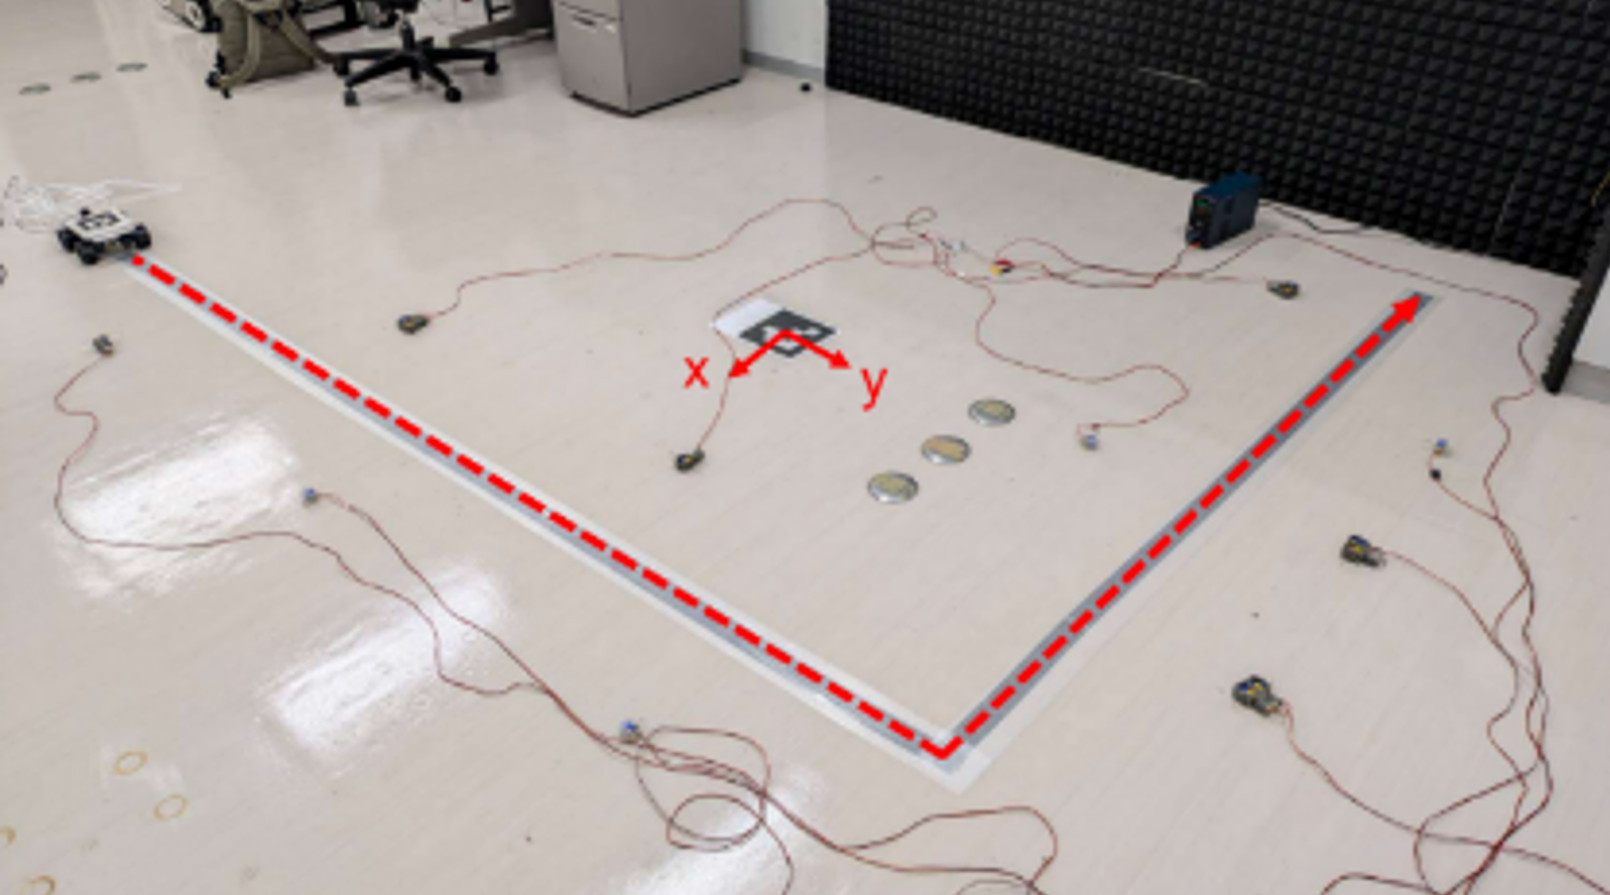
\includegraphics[keepaspectratio, width=1.0\linewidth]{chap4/env_experiment.png}
  \caption{実験環境}
  \label{fig:exp_setup}
\end{figure}

\begin{figure}[t]
  \centering
  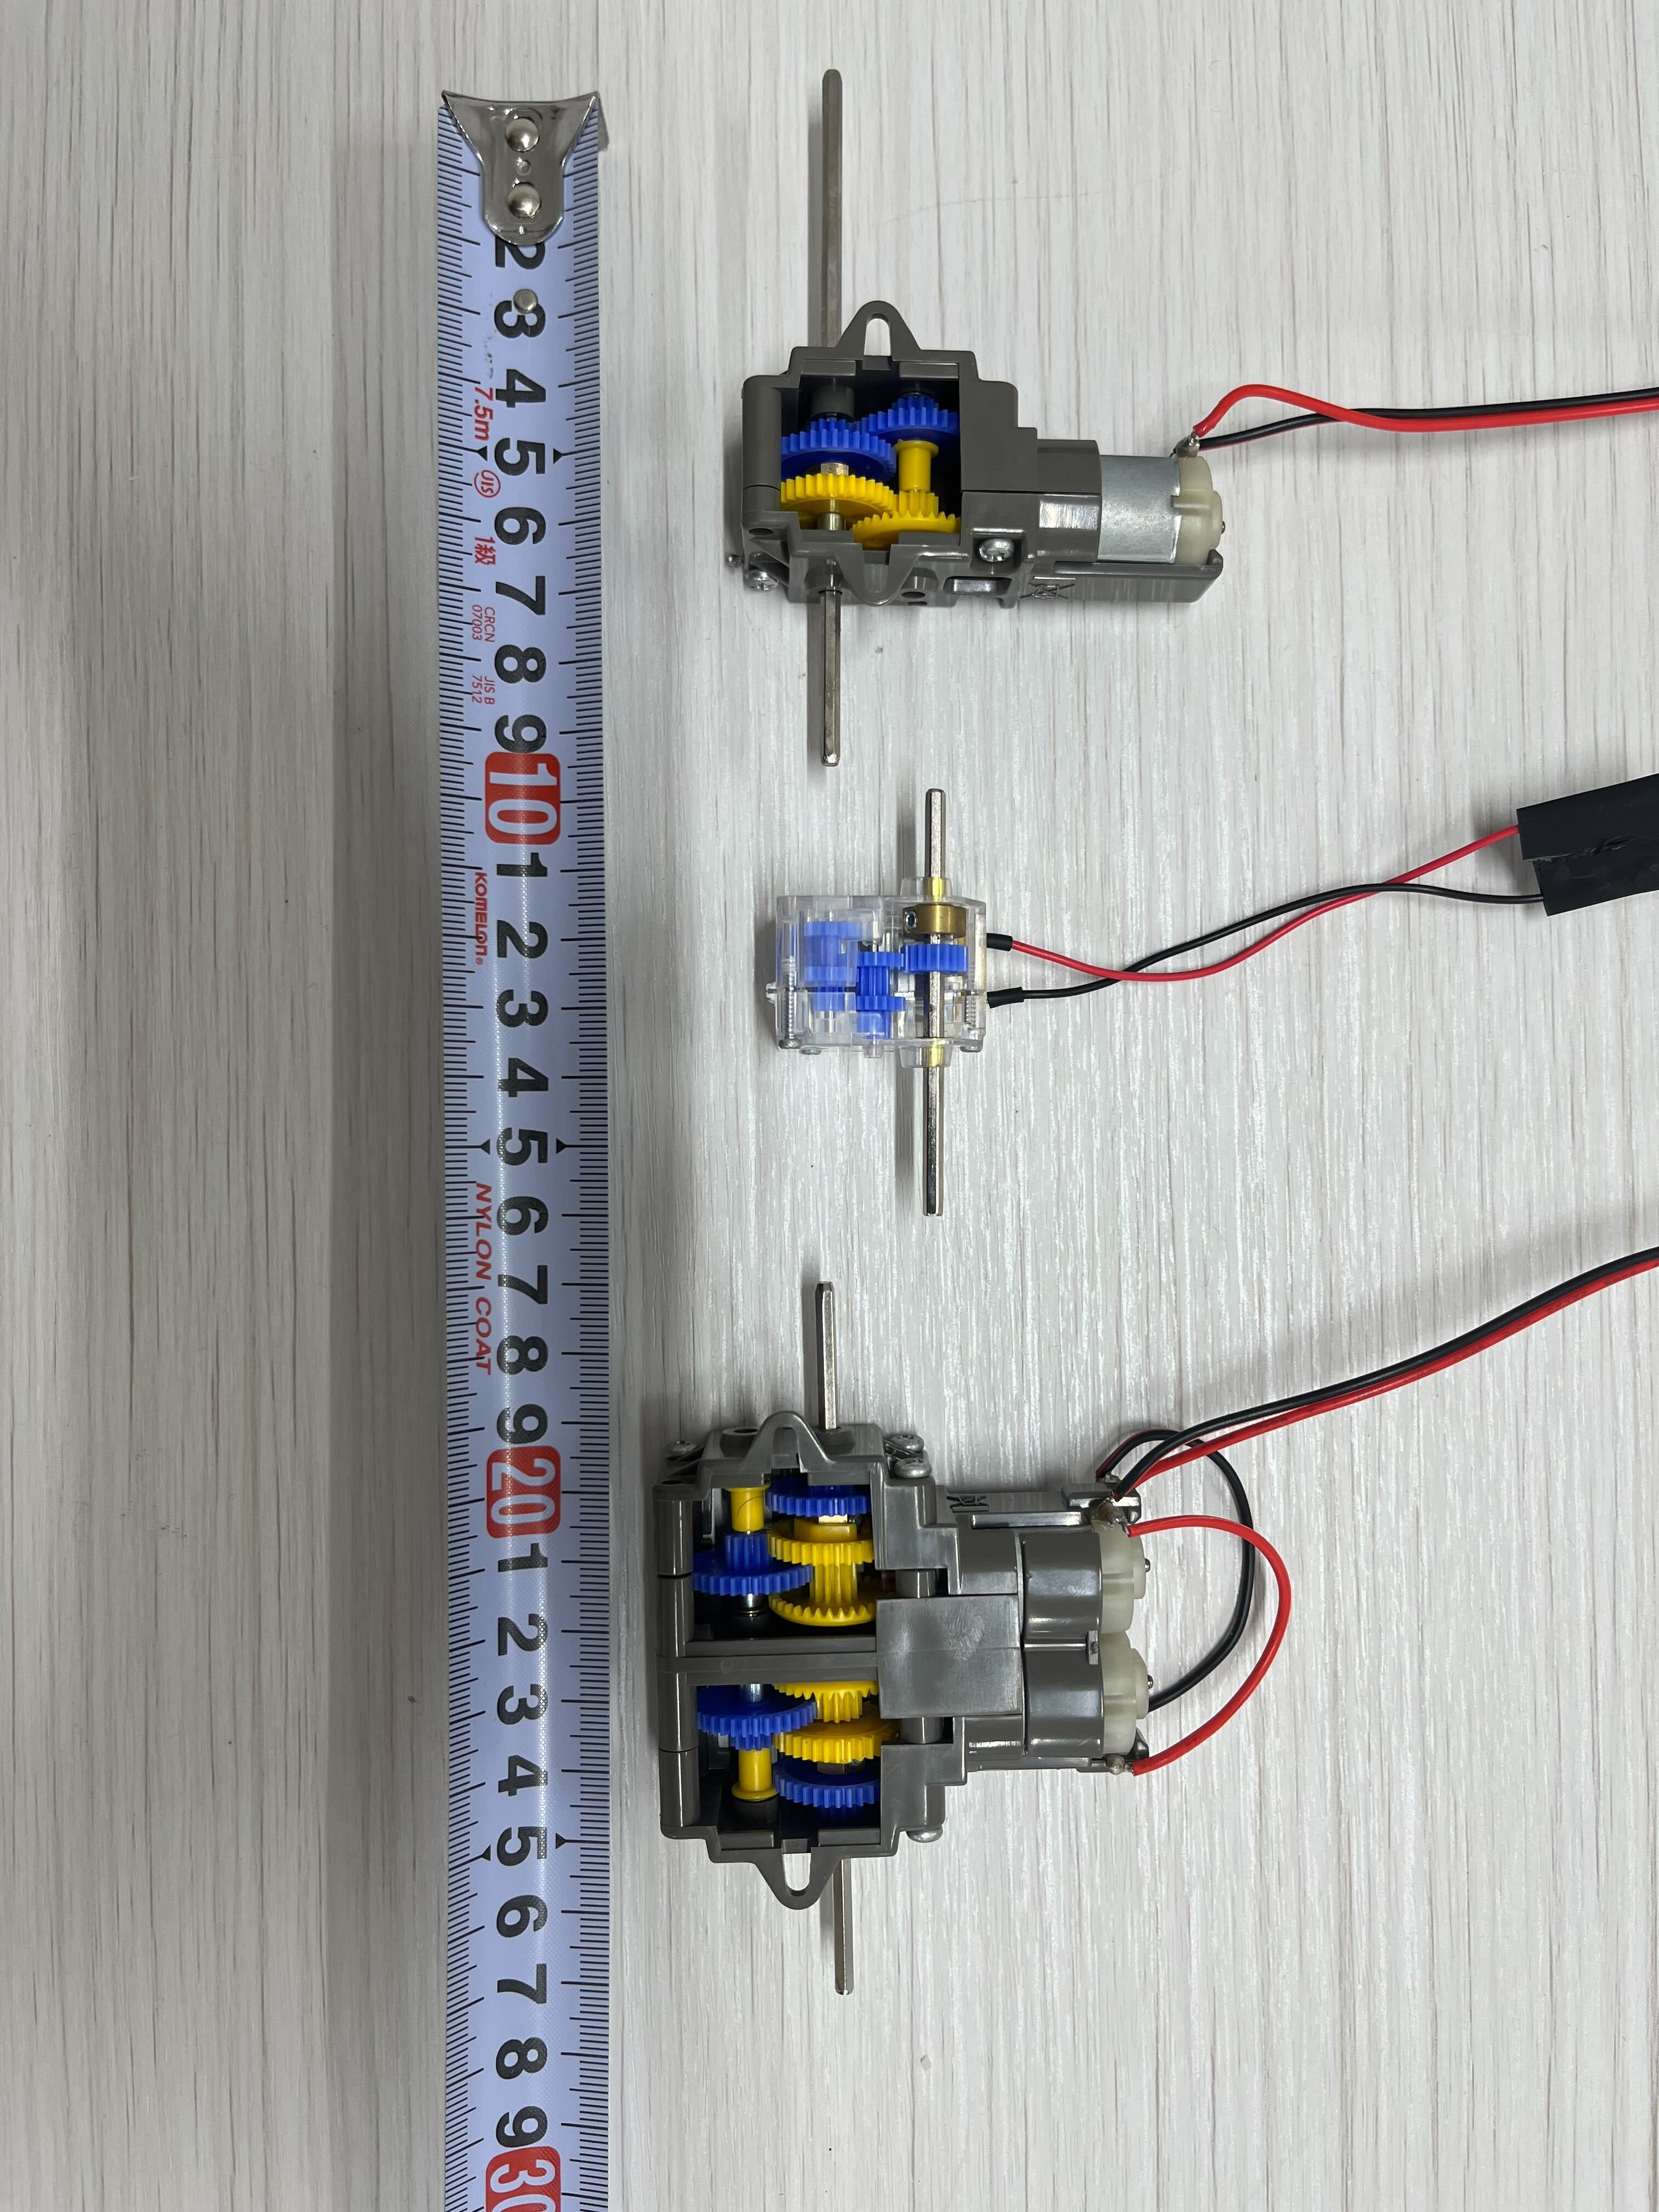
\includegraphics[angle=90,keepaspectratio, width=1.0\linewidth]{chap4/gearbox.jpg}
  \caption{音源のギアボックス}
  \label{fig:gearbox}
\end{figure}

\end{document}
